\setlength{\columnsep}{3pt}
\begin{flushleft}

\bigskip

\begin{itemize}
	\item SSH stand for \textbf{S}ecure \textbf{SH}ell.
	\item SSH allows secure \textbf{remote access} to Linux server.
	\item It provides a \textbf{secure and encrypted communication over a network}.
	
	\begin{figure}[h!]
		\centering
		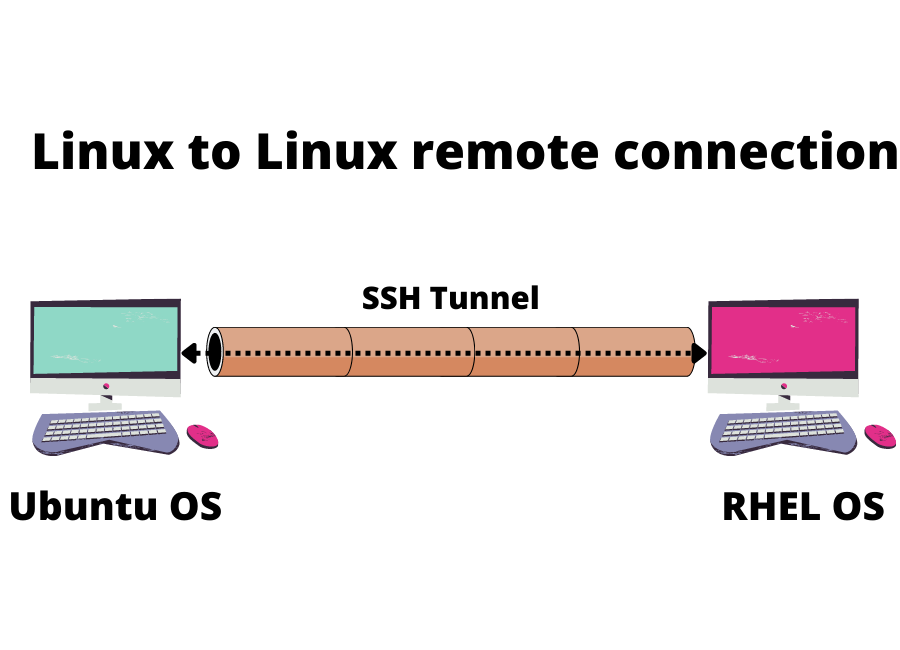
\includegraphics[scale=0.45]{content/chapter19/images/ssh.png}
			\caption{SSH connection}
		\label{fig:boot1}
	\end{figure}

	\item Types of SSH connection:
	\begin{itemize}
		\item Password based SSH
		\item Passwordless or Key based SSH
	\end{itemize}
	
	We shall see more on this in the coming sections.
	
	
\end{itemize}
 


\end{flushleft}
\newpage


